% BUDGET: 1.3 pages — the core section of a Demo Track paper

\begin{figure}[b]
	\centering
	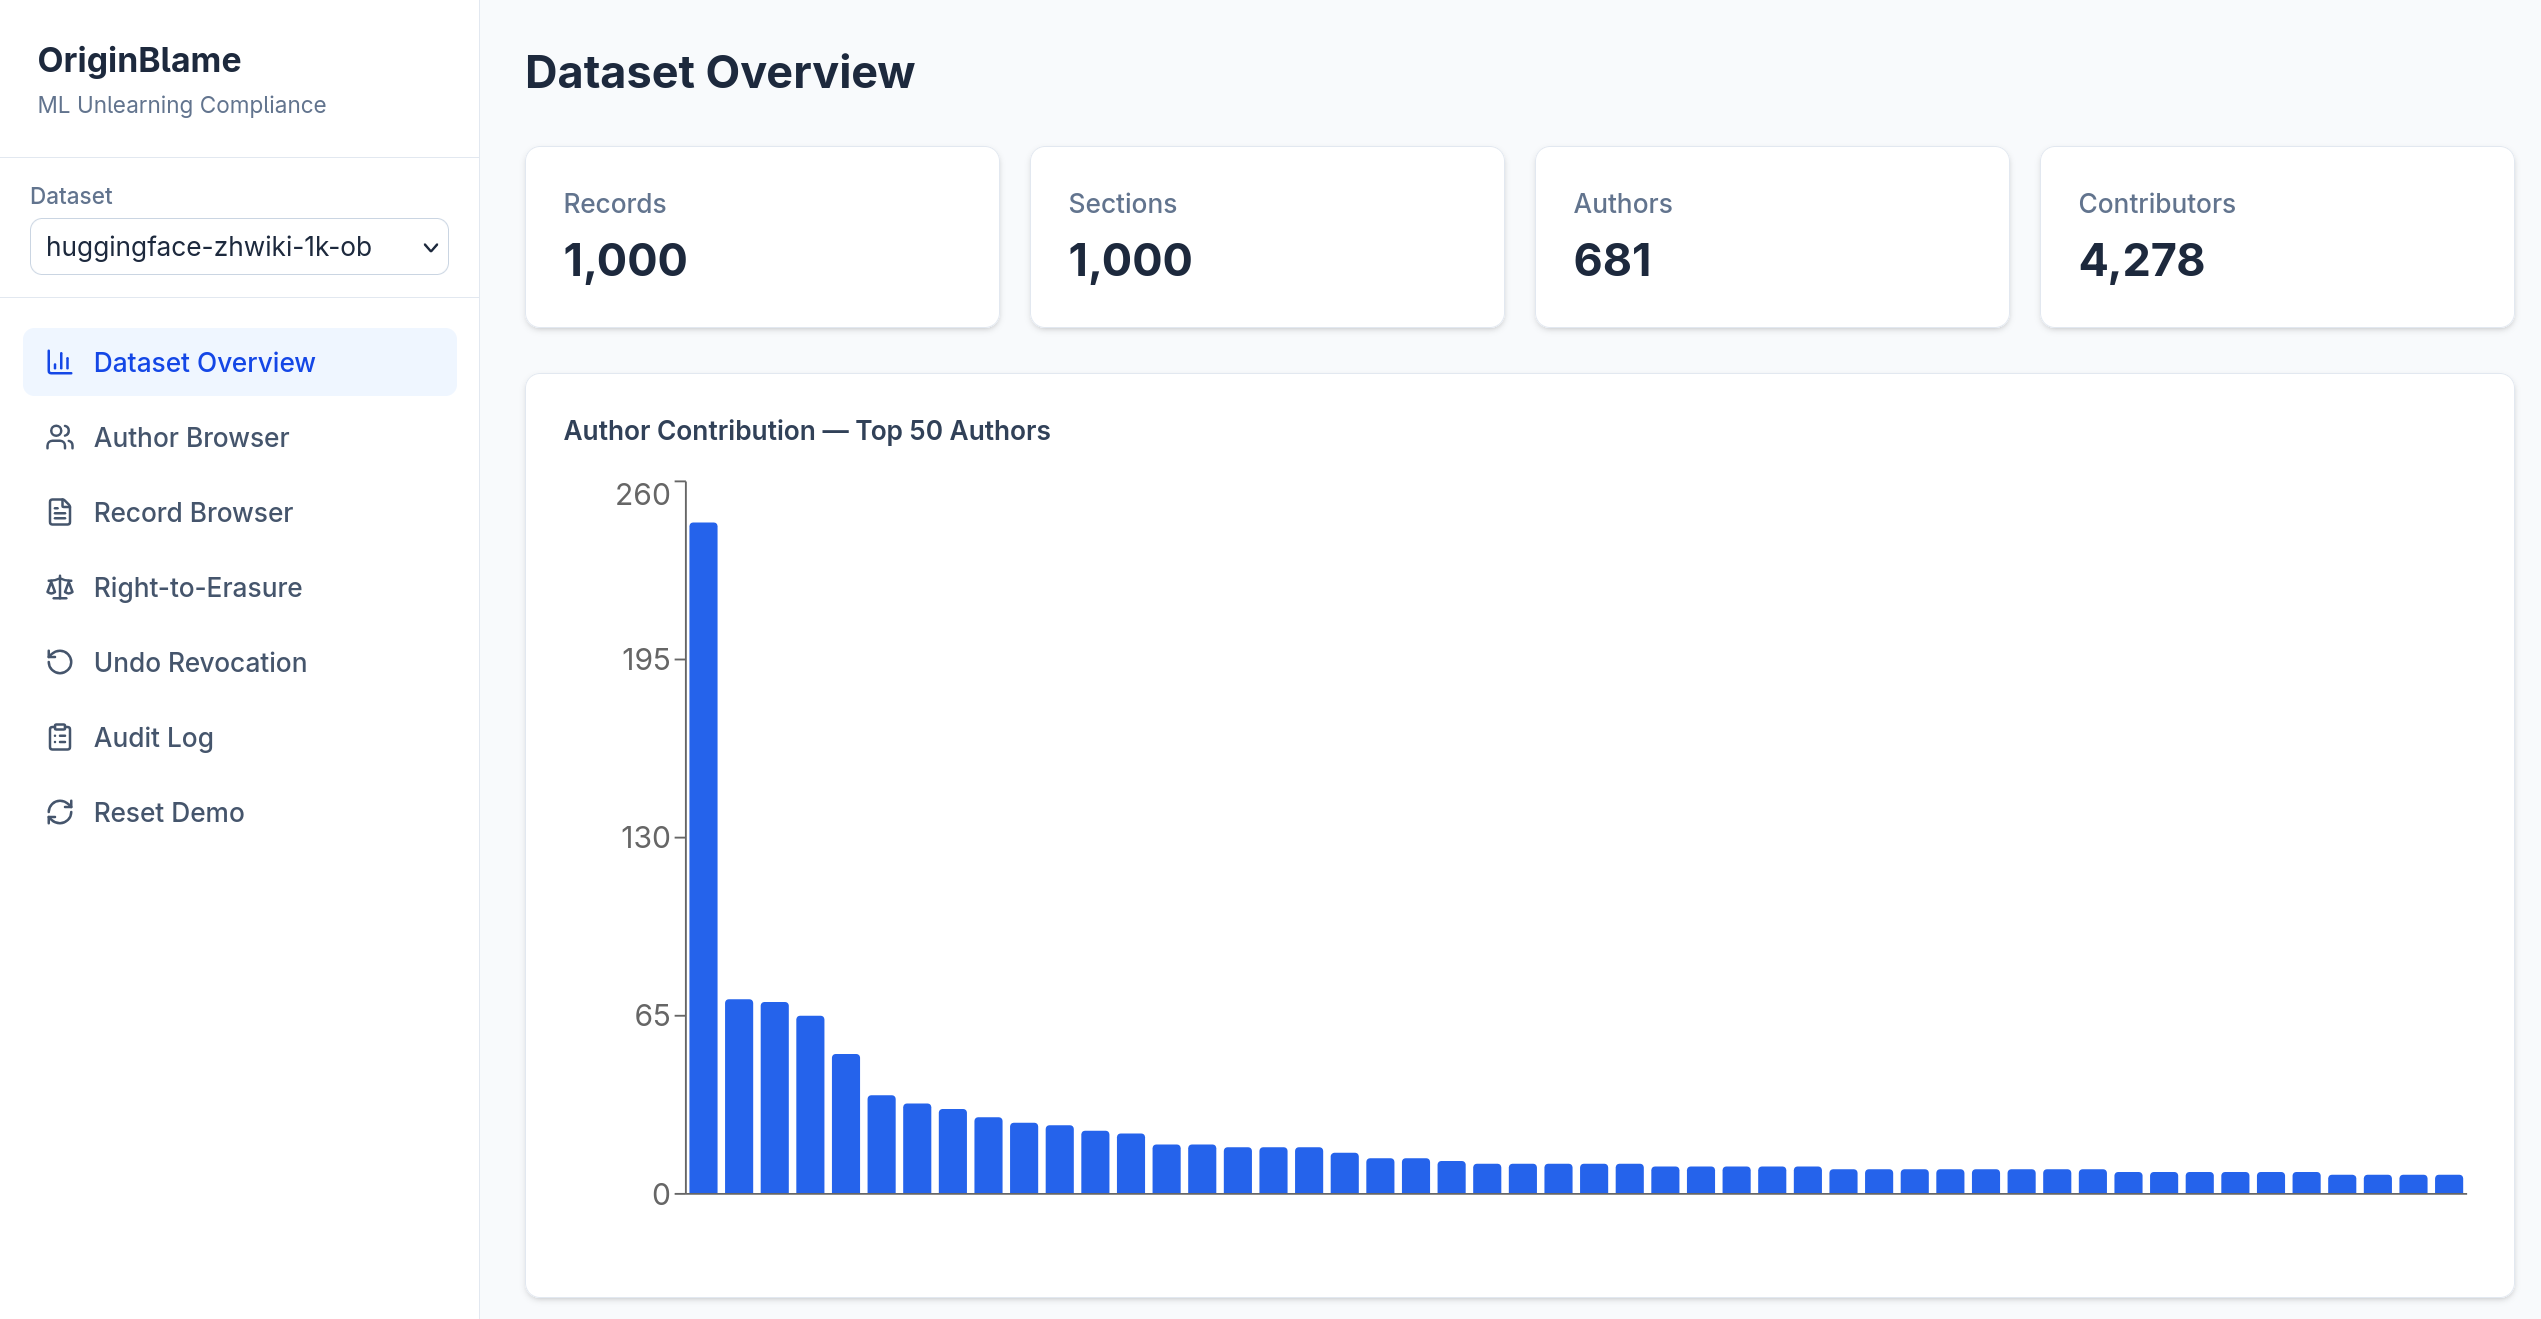
\includegraphics[width=\columnwidth]{figures-cikm/webapp-screenshot}
	\Description{Screenshot of the OriginBlame web application showing the Dataset Overview page with author distribution chart and statistics.}
	\caption{Dataset Overview page showing 1,000 Wikipedia records, 681 authors, 4,278 contributors, and the top-50 author contribution chart.}
	\label{fig:webapp}
\end{figure}

\section{Demonstration}

\subsection{Intended Audience}

The demonstration targets data engineers, ML researchers, and compliance officers. No prior knowledge is assumed.

\subsection{Web Interface}

The demonstration runs as a FastAPI + React web application. The webapp auto-discovers all eight available OB-indexed datasets spanning three dimensions: (1)~\textbf{Chinese Wikipedia} at four scales (1k--323k records, 681--46.7k authors, 4.3k--482k contributors), (2)~\textbf{Linux kernel source} at three scales (1k--66k records, 1.8k--22.8k authors, git-blame attribution), and (3)~\textbf{ChatML instruction data} (36k Q\&A pairs, 2.7k authors, 17k contributors). Users can switch datasets at any time to compare provenance across domains, scales, and pipeline stages.

The interface provides seven views via sidebar navigation:

\begin{itemize}
	\item \textbf{Dataset Overview} (Figure~\ref{fig:webapp}): summary statistics, top-50 author contribution chart, paginated author table. On the 1k zhwiki dataset, attendees observe a skewed distribution (681 authors, 4,278 contributors, top author holds 24.5\%). Switching to ChatML and kernel datasets reveals cross-domain generalization---the same author shows 3,618 sections on ChatML, and git-blame attributes 1,779 Linux kernel authors.
	\item \textbf{Author Browser} (Figure~\ref{fig:author-browser}): searchable author table; clicking an author reveals metrics and a paginated record list. Attendees can trace any record's full provenance chain (line\_hash $\rightarrow$ section\_hash $\rightarrow$ author $\rightarrow$ license) in under 4\,ms via the hash-sharded index.
	\item \textbf{Record Browser} (Figure~\ref{fig:record-browser}): paginated record list (title, heading, preview, authors, year, status) alongside a detail panel showing the full provenance chain---document hash, section hash with path, registered authors vs.\ all contributors, license, and the complete ChatML text of the selected record.
	\item \textbf{Right-to-Erasure} (Figure~\ref{fig:erasure}): guided three-level revocation (author / section / record). On ChatML, revoking author ``Ohtashinichiro'' (541 sections, 1{,}951 records) shows that dataset-level deletion would destroy 9{,}951 sections, while record-level provenance targets only 541---an 18.4$\times$ reduction. At 10k scale, over-deletion ranges from 2.8$\times$ to 44.8$\times$ (Table~\ref{tab:revocation}).
	\item \textbf{Undo Revocation}: reverses any prior revocation with one click, leveraging ob's lazy tag-cascade design for instant restoration.
	\item \textbf{Audit Log}: timestamped trail of all state-changing operations, filterable by type---providing compliance evidence for GDPR Article~17~\cite{gdpr2016} (right to erasure) or copyright audits.
	\item \textbf{Reset Demo}: restores the dataset to its initial state for the next attendee.
\end{itemize}

\begin{figure}[t]
	\centering
	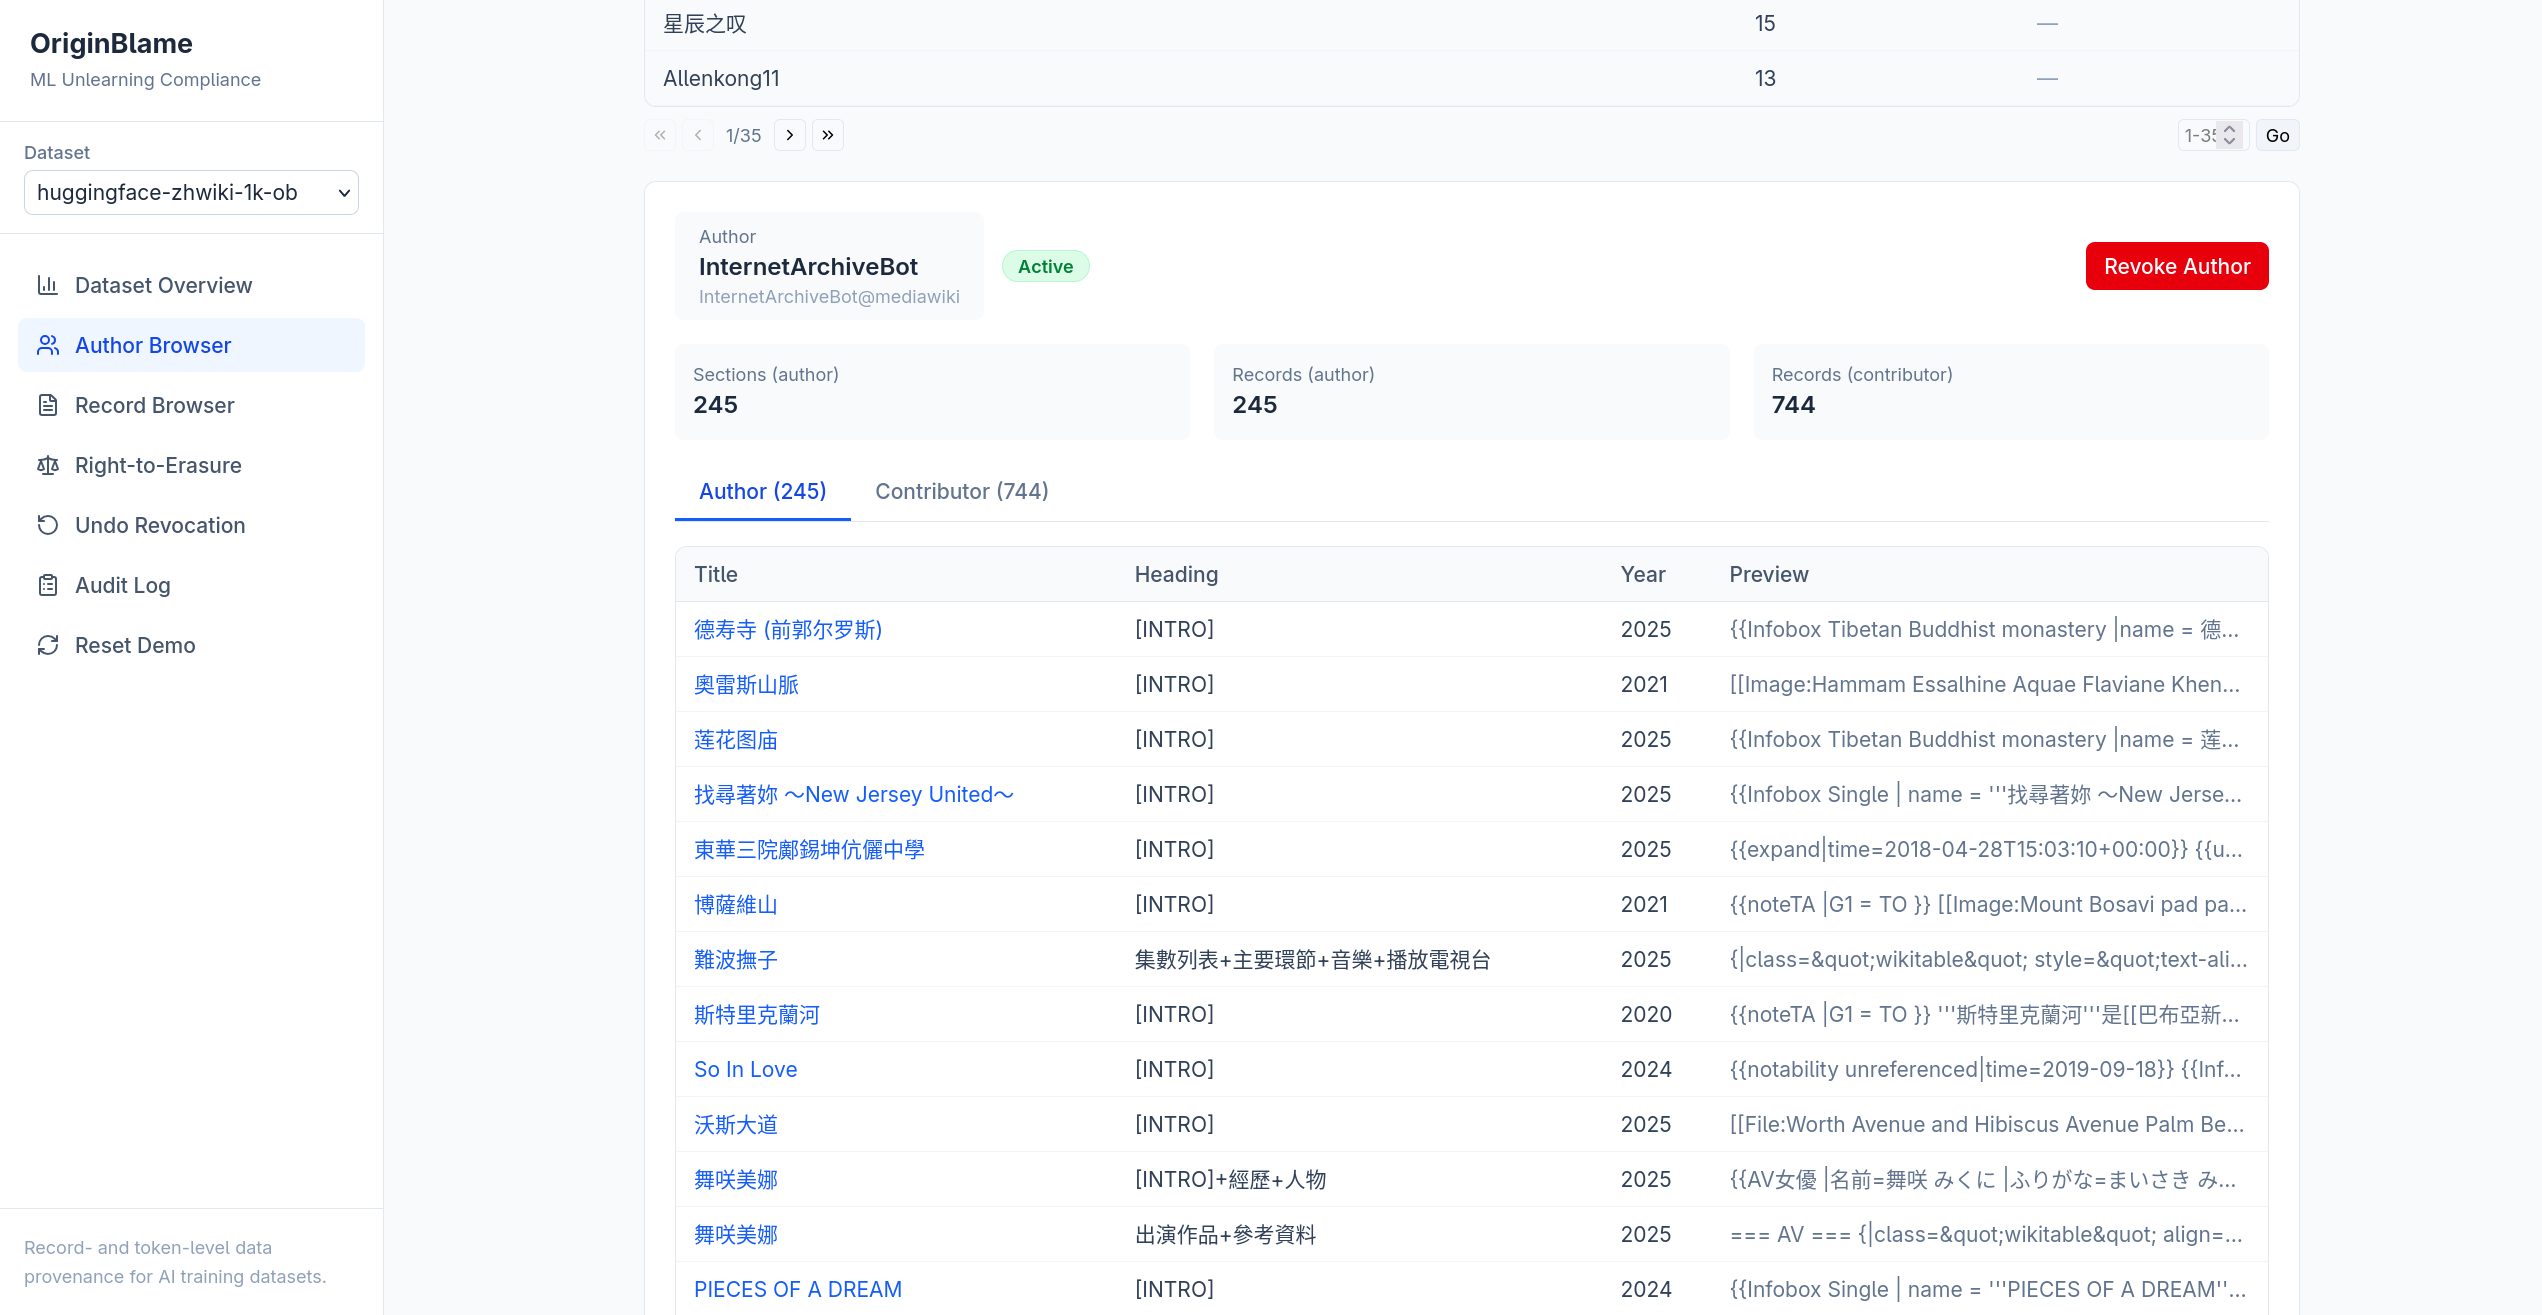
\includegraphics[width=\columnwidth]{figures-cikm/webapp-author-browser}
	\Description{Screenshot of the Author Browser page showing author detail panel with sections, records as author vs.\ contributor, and a paginated record list.}
	\caption{Author Browser on the ChatML dataset: InternetArchiveBot detail showing 3,618 sections, 12,981 records as author vs.\ 30,979 as contributor.}
	\label{fig:author-browser}
\end{figure}

\begin{figure}[t]
	\centering
	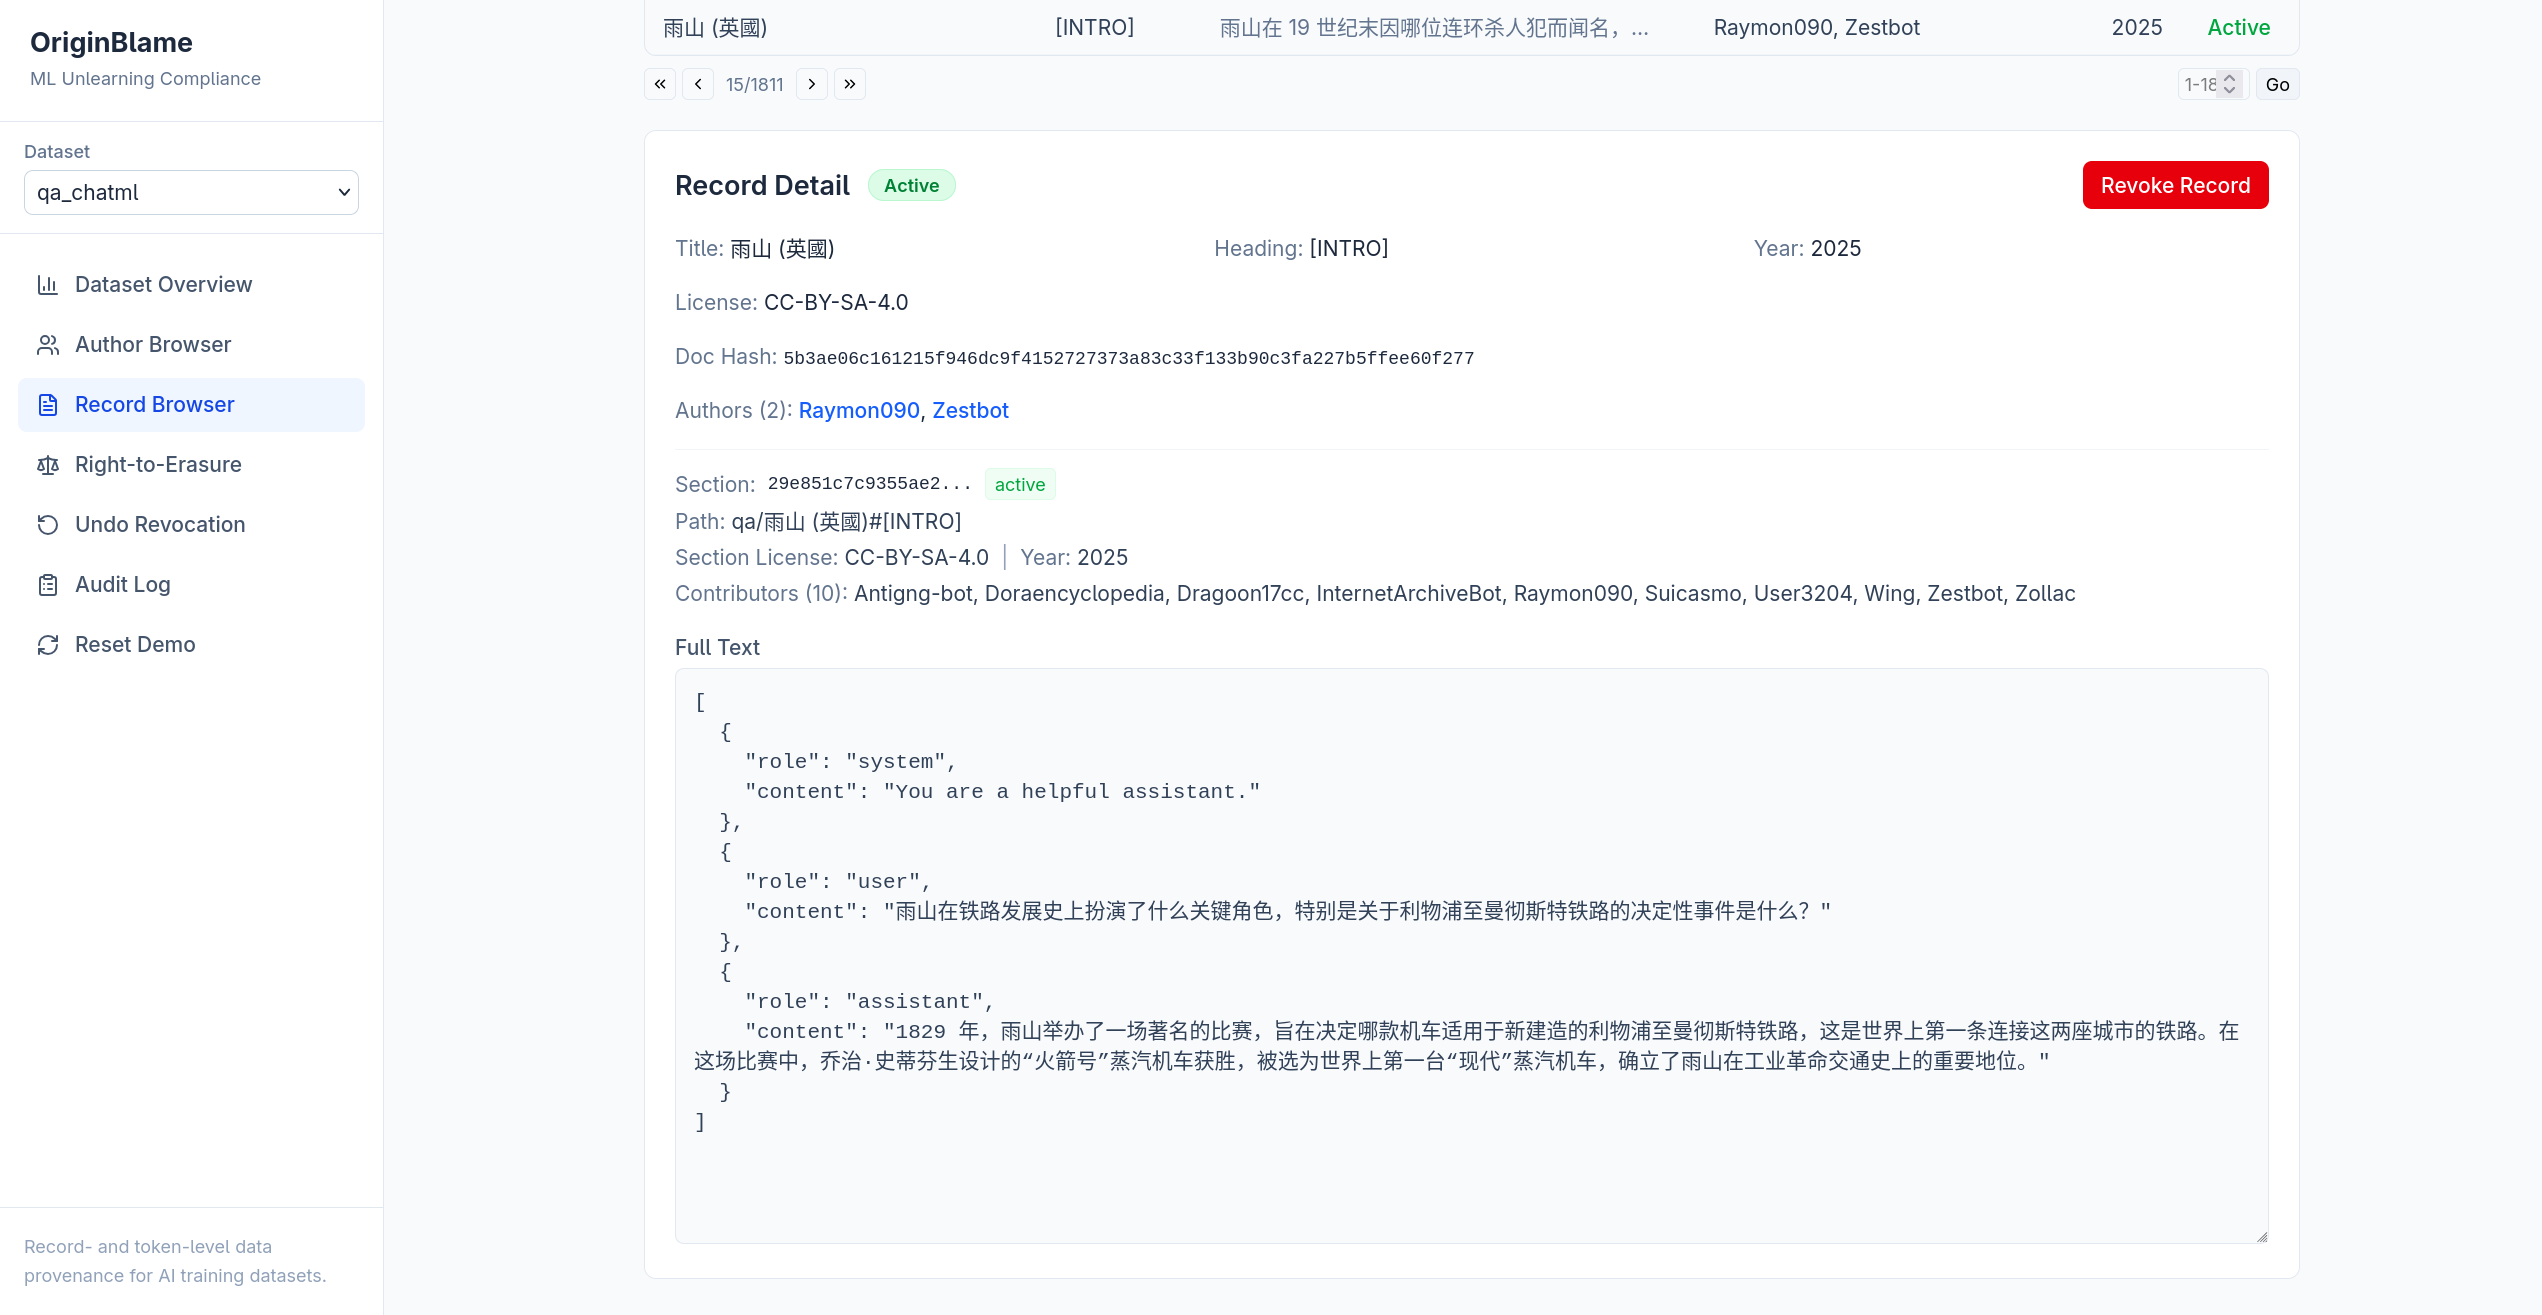
\includegraphics[width=\columnwidth]{figures-cikm/webapp-records-list}
	\Description{Screenshot of the Record Browser page showing a record detail panel with document hash, section hash, registered authors, contributors, license, and the full ChatML text.}
	\caption{Record Browser detail view showing doc hash, section hash with path, registered authors vs.\ contributors, CC-BY-SA-4.0 license, and full record text.}
	\label{fig:record-browser}
\end{figure}

\subsection{CLI Demonstrations}

Beyond the web interface, the \texttt{ob} CLI demonstrates token-level provenance---capabilities not yet exposed in the webapp. Attendees can run \texttt{ob show -{}-author NAME -{}-tokenizer gpt2} to query an author's token contribution, \texttt{ob revoke -{}-author NAME -{}-tokenizer gpt2} for token-level revocation, and \texttt{ob generate-set -{}-tokenizer gpt2 -o forget.bin} to export the forget set for unlearning algorithms.

\subsection{Video and Availability}

A 3-minute demonstration video is available at \url{https://youtu.be/vM3pdSRkke8}. The live demo is accessible at \url{https://ob.organism.org.cn}.

\begin{figure}[t]
	\centering
	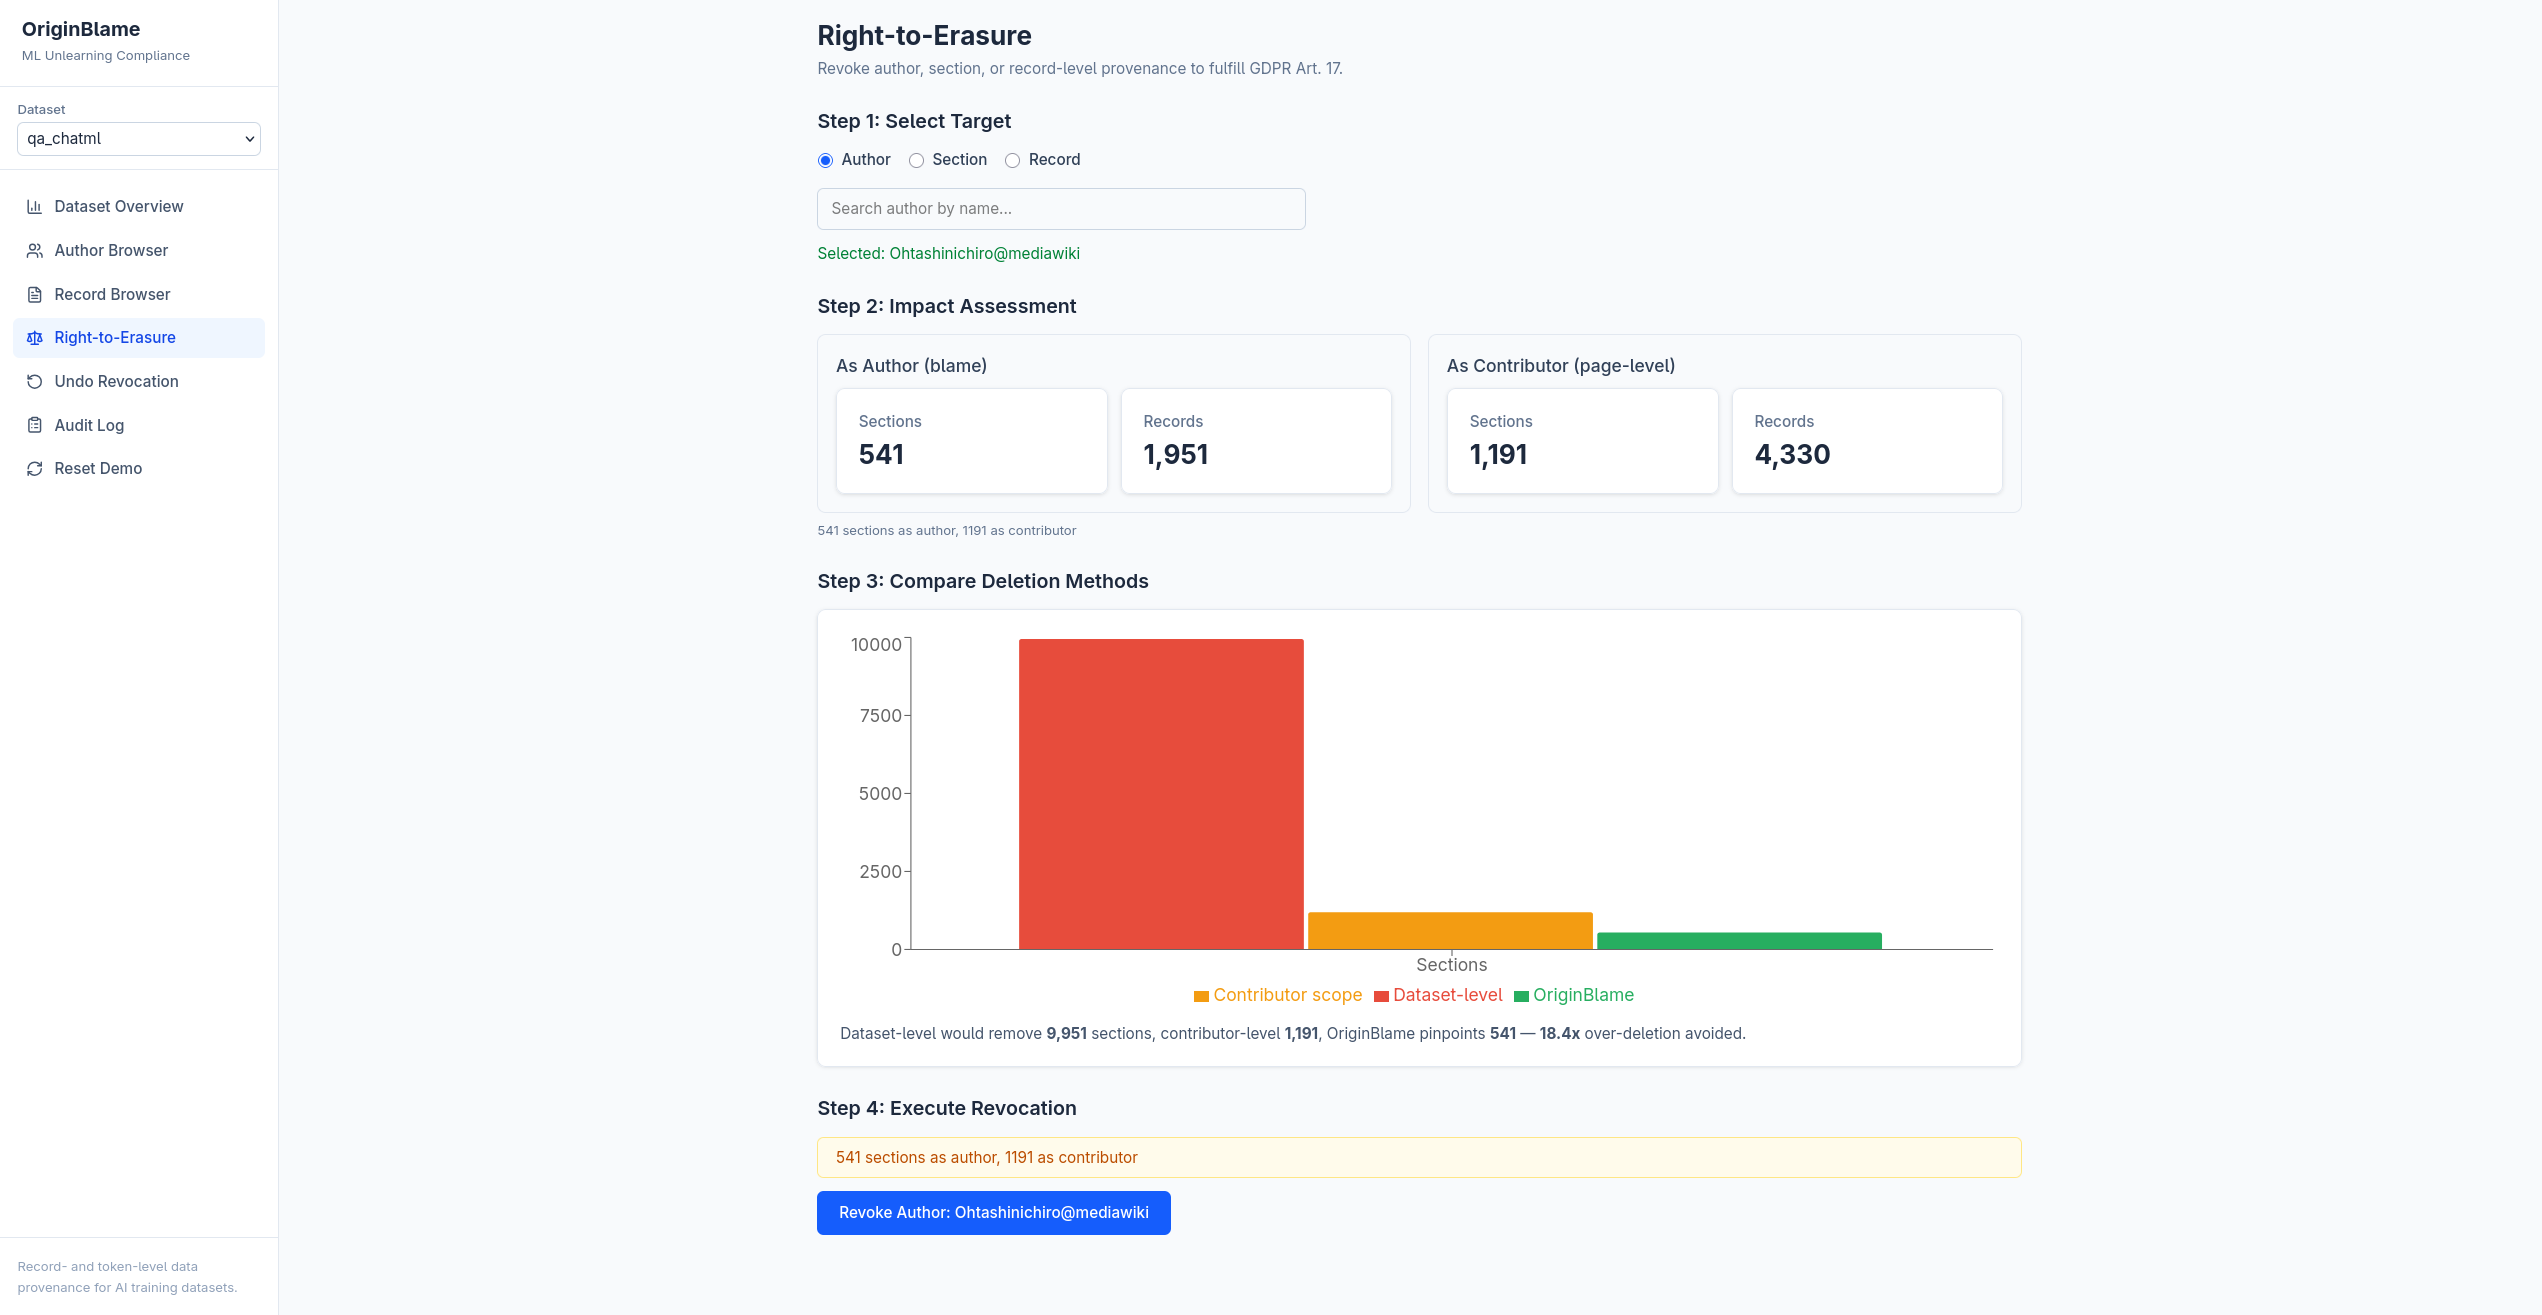
\includegraphics[width=\columnwidth]{figures-cikm/webapp-erasure}
	\Description{Screenshot of the Right-to-Erasure page showing impact assessment and comparison bar chart for author-level revocation.}
	\caption{Right-to-Erasure on the ChatML dataset: revoking Ohtashinichiro. The comparison chart shows dataset-level deletion (9,951) vs.\ contributor-level reference (1,191; ob tracks contributors but does not expose contributor-level revocation) vs.\ author-scope (541)---18.4$\times$ over-deletion avoided.}
	\label{fig:erasure}
\end{figure}
